\documentclass[10pt,a4paper]{article}

\usepackage[a4paper, top=0.9cm, bottom=0.9cm, left=1cm, right=1cm]{geometry}
\usepackage{graphicx}
\usepackage{float}
\usepackage{amsmath}
\usepackage{amssymb}
\usepackage{xcolor}
\usepackage{mdframed}
\usepackage{parskip}
\usepackage{enumitem}
\usepackage{titlesec}
\usepackage{booktabs}
\usepackage{array}
\usepackage{tikz}
\usetikzlibrary{arrows.meta, positioning}
\usepackage[T1]{fontenc}

\graphicspath{{../../Slides/}}

\definecolor{keyblue}{RGB}{30, 80, 160}
\definecolor{keybluebg}{RGB}{220, 235, 255}
\definecolor{noteorange}{RGB}{200, 100, 0}
\definecolor{noteorangebg}{RGB}{255, 240, 215}
\definecolor{warnred}{RGB}{180, 30, 30}
\definecolor{warnredbg}{RGB}{255, 220, 220}
\definecolor{defgreen}{RGB}{20, 110, 50}
\definecolor{defgreenbg}{RGB}{215, 245, 225}
\definecolor{headernavy}{RGB}{25, 35, 90}

\newmdenv[linecolor=keyblue,backgroundcolor=keybluebg,linewidth=1.5pt,
  leftline=true,rightline=false,topline=false,bottomline=false,
  innerleftmargin=6pt,innerrightmargin=5pt,
  innertopmargin=2pt,innerbottommargin=2pt,
  skipabove=2pt,skipbelow=2pt]{keybox}

\newmdenv[linecolor=noteorange,backgroundcolor=noteorangebg,linewidth=1.5pt,
  leftline=true,rightline=false,topline=false,bottomline=false,
  innerleftmargin=6pt,innerrightmargin=5pt,
  innertopmargin=2pt,innerbottommargin=2pt,
  skipabove=2pt,skipbelow=2pt]{notebox}

\newmdenv[linecolor=defgreen,backgroundcolor=defgreenbg,linewidth=1.5pt,
  leftline=true,rightline=false,topline=false,bottomline=false,
  innerleftmargin=6pt,innerrightmargin=5pt,
  innertopmargin=2pt,innerbottommargin=2pt,
  skipabove=2pt,skipbelow=2pt]{defbox}

\newmdenv[linecolor=warnred,backgroundcolor=warnredbg,linewidth=1.5pt,
  leftline=true,rightline=false,topline=false,bottomline=false,
  innerleftmargin=6pt,innerrightmargin=5pt,
  innertopmargin=2pt,innerbottommargin=2pt,
  skipabove=2pt,skipbelow=2pt]{warnbox}

\titleformat{\section}[block]{\normalsize\bfseries\color{headernavy}}{}{0pt}{}
  [\vspace{1pt}\rule{\linewidth}{0.6pt}\vspace{1pt}]
\titleformat{\subsection}[block]{\small\bfseries\color{keyblue}}{}{0pt}{}
\titlespacing*{\section}{0pt}{4pt}{1pt}
\titlespacing*{\subsection}{0pt}{2pt}{1pt}

\setlist{nosep, topsep=0pt, itemsep=0pt, leftmargin=1.2em}
\parskip=1pt
\parindent=0pt

% ===========================================================================
\begin{document}
% ===========================================================================

\begin{center}
  {\large\bfseries\color{headernavy} Q9 \textemdash{} Fault Detection via Hidden Markov Models}\\[1pt]
  {\small MM11 $\cdot$ Hans-Peter Schwefel}
\end{center}
\vspace{1pt}\hrule height 1pt\vspace{3pt}

% ===========================================================================
\section*{1\quad Fault-Detector Metrics: Confusion Matrix}
% ===========================================================================
\begin{defbox}
\textbf{Fault-detector} $\mathrm{fd}(t)$: function taking system observations $o(t)$ as input, outputting a conjecture of whether a fault is present (binary: $\mathrm{FD}{=}1$ fault, $\mathrm{FD}{=}0$ no fault).\\[2pt]
Input $o(t)$ can be a \textbf{single observation} or a \textbf{sequence} of past observations --- you define.\\[2pt]
System has 2 true states: $S{=}0$ (normal) and $S{=}1$ (faulty) $\Rightarrow$ 4 outcome combinations (confusion matrix below).
\end{defbox}
\vspace{3pt}

% Confusion matrix (larger, full-width left) + summary right
\vspace{0pt}
\begin{minipage}[t]{0.57\textwidth}
\vspace{0pt}
\begin{center}
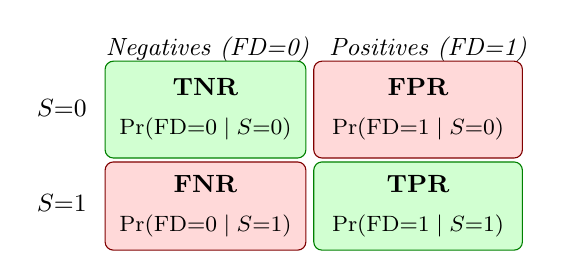
\begin{tikzpicture}[font=\small]
  % Column headers
  \node[font=\small\itshape] at (1.95, 2.1)  {Negatives (FD=0)};
  \node[font=\small\itshape] at (4.75, 2.1)  {Positives (FD=1)};
  % Row labels
  \node[font=\small\bfseries] at (0.1, 1.35) {$S{=}0$};
  \node[font=\small\bfseries] at (0.1, 0.15) {$S{=}1$};
  % TNR
  \draw[fill=green!18, draw=green!50!black, rounded corners=3pt]
    (0.65, 0.72) rectangle (3.2, 1.95);
  \node[font=\small, align=center] at (1.925, 1.335)
    {\textbf{TNR}\\[3pt]\footnotesize$\Pr(\mathrm{FD}{=}0\mid S{=}0)$};
  % FPR
  \draw[fill=red!15, draw=red!50!black, rounded corners=3pt]
    (3.3, 0.72) rectangle (5.95, 1.95);
  \node[font=\small, align=center] at (4.625, 1.335)
    {\textbf{FPR}\\[3pt]\footnotesize$\Pr(\mathrm{FD}{=}1\mid S{=}0)$};
  % FNR
  \draw[fill=red!15, draw=red!50!black, rounded corners=3pt]
    (0.65, -0.45) rectangle (3.2, 0.67);
  \node[font=\small, align=center] at (1.925, 0.11)
    {\textbf{FNR}\\[3pt]\footnotesize$\Pr(\mathrm{FD}{=}0\mid S{=}1)$};
  % TPR
  \draw[fill=green!18, draw=green!50!black, rounded corners=3pt]
    (3.3, -0.45) rectangle (5.95, 0.67);
  \node[font=\small, align=center] at (4.625, 0.11)
    {\textbf{TPR}\\[3pt]\footnotesize$\Pr(\mathrm{FD}{=}1\mid S{=}1)$};
\end{tikzpicture}
\end{center}
\end{minipage}\hfill
\begin{minipage}[t]{0.40\textwidth}
\vspace{0pt}
\begin{notebox}
\small $\mathrm{TNR} + \mathrm{FPR} = 1$\\[2pt]
$\mathrm{FNR} + \mathrm{TPR} = 1$\\[4pt]
\textbf{Accuracy:}
\[ \mathrm{Acc} = \mathrm{TPR}{\cdot}\Pr(S{=}1) + \mathrm{TNR}{\cdot}\Pr(S{=}0) \]
Depends on how often system is faulty.
\end{notebox}
\vspace{2pt}
\end{minipage}

\vspace{3pt}

\vspace{2pt}

% ===========================================================================
\section*{2\quad Example: Congestion Detection \& ROC Curve}
% ===========================================================================

Congestion detector: $\mathrm{FD}(t_i)=\mathbf{1}(\mathrm{RTT}_i > \gamma)$ --- declare congestion ($\mathrm{FD}{=}1$) when RTT exceeds threshold $\gamma$, normal ($\mathrm{FD}{=}0$) otherwise.

\vspace{3pt}

% --- Row 1: RTT example (left) + explanation (right) ---
\vspace{0pt}
\begin{minipage}[t]{0.50\textwidth}
\vspace{0pt}
\includegraphics[page=10, width=\linewidth, trim=35 30 35 110, clip]{2026_MM11_Fault_Detection_HMM.pdf}
\end{minipage}\hfill
\begin{minipage}[t]{0.47\textwidth}
\vspace{0pt}
\begin{keybox}
\textbf{Congestion detector:} $\mathrm{FD}(t_i)=\mathbf{1}(\mathrm{RTT}_i > \gamma)$\\[3pt]
RTT distributions for $S{=}0$ (normal) and $S{=}1$ (fault) \textbf{overlap} $\Rightarrow$ no perfect threshold exists.\\[3pt]
At $\gamma{=}55$\,ms (dashed line):\\
\begin{itemize}
  \item Left of $\gamma$: FD$=$0 $\Rightarrow$ \textbf{TN} (if $S{=}0$) or \textbf{FN} (if $S{=}1$)
  \item Right of $\gamma$: FD$=$1 $\Rightarrow$ \textbf{FP} (if $S{=}0$) or \textbf{TP} (if $S{=}1$)
\end{itemize}
\vspace{2pt}
Moving $\gamma$ right: FPR$\downarrow$ \textbf{and} TPR$\downarrow$ simultaneously.
\end{keybox}
\end{minipage}

\vspace{4pt}

To set $\gamma$ precisely we can use the \textbf{ROC curve} --- sweeping $\gamma$ traces a curve in (FPR, TPR) space, letting us choose the best operating point for the required trade-off.

\vspace{3pt}

% --- Row 2: ROC curve (left) + ROC keybox (right) ---
\vspace{0pt}
\begin{minipage}[t]{0.50\textwidth}
\vspace{0pt}
\includegraphics[page=11, height=5.5cm, trim=310 50 15 125, clip]{2026_MM11_Fault_Detection_HMM.pdf}
\end{minipage}\hfill
\begin{minipage}[t]{0.47\textwidth}
\vspace{0pt}
\begin{keybox}
\textbf{ROC (Receiver Operating Characteristic):}\\
sweep $\gamma \Rightarrow$ plot (FPR, TPR) pairs.\\[4pt]
\begin{itemize}
  \item \textbf{$(0,1)$ top-left}: ideal --- TPR$=$1, FPR$=$0
  \item \textbf{Diagonal}: random guess (useless)
  \item \textbf{$\gamma^{\text{MPE}}{=}54.9$\,ms}: min.\ prob.\ error point
  \item Choose $\gamma$ on curve to match required FPR/TPR trade-off
\end{itemize}
\end{keybox}
\end{minipage}

\vspace{2pt}

% ===========================================================================
\clearpage
\section*{Why we use HMM (Need to model uncertiantiy of fault knowledge)}
% ===========================================================================
\textbf{Why HMM?} The true system state (faulty/normal) is \textbf{not directly observable} --- we only ever get indirect measurements such as RTT. We must therefore \textbf{infer} the hidden fault state purely from these observations. \\[4pt]

HMM formalises exactly this: a hidden Markov state evolves over time, emitting observable symbols --- allowing us to estimate the most likely underlying fault state from what we can actually measure.

\section*{3\quad HMM Definition: $\langle E,\,V,\,\underline{\pi}_1,\,\underline{P},\,\underline{B}\rangle$}

Example: we can only observe whether a packet was received correctly or with error ($c$/$e$) --- we want to determine the hidden wireless link state (good, intermediate, poor).

\vspace{4pt}

% --- Row 1: large TikZ (left) + emission table (right) ---
\vspace{0pt}
\begin{minipage}[t]{0.54\textwidth}
\vspace{0pt}
\begin{center}
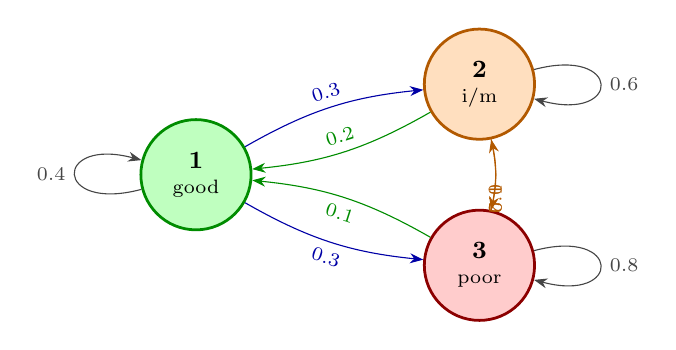
\begin{tikzpicture}[>=Stealth, font=\small]
  \node[draw, circle, fill=green!25, draw=green!55!black, line width=1pt,
        minimum size=1.4cm, align=center] (s1) at (0,0) {\textbf{1}\\[-2pt]\scriptsize good};
  \node[draw, circle, fill=orange!25, draw=orange!70!black, line width=1pt,
        minimum size=1.4cm, align=center] (s2) at (3.6,1.15) {\textbf{2}\\[-2pt]\scriptsize i/m};
  \node[draw, circle, fill=red!20, draw=red!55!black, line width=1pt,
        minimum size=1.4cm, align=center] (s3) at (3.6,-1.15) {\textbf{3}\\[-2pt]\scriptsize poor};
  % Self loops
  \draw[->, gray!55!black] (s1) to[loop left, looseness=8] node[left, font=\scriptsize]{$0.4$} (s1);
  \draw[->, gray!55!black] (s2) to[loop right, looseness=8] node[right, font=\scriptsize]{$0.6$} (s2);
  \draw[->, gray!55!black] (s3) to[loop right, looseness=8] node[right, font=\scriptsize]{$0.8$} (s3);
  % 1→2, 1→3
  \draw[->, blue!65!black] (s1) to[bend left=12] node[sloped, above, font=\scriptsize]{$0.3$} (s2);
  \draw[->, blue!65!black] (s1) to[bend right=12] node[sloped, below, font=\scriptsize]{$0.3$} (s3);
  % 2→1, 2→3
  \draw[->, green!55!black] (s2) to[bend left=12] node[sloped, above, font=\scriptsize]{$0.2$} (s1);
  \draw[->, orange!70!black] (s2) to[bend left=12] node[sloped, right, font=\scriptsize]{$0.2$} (s3);
  % 3→1, 3→2
  \draw[->, green!55!black] (s3) to[bend right=12] node[sloped, below, font=\scriptsize]{$0.1$} (s1);
  \draw[->, orange!70!black] (s3) to[bend right=12] node[sloped, left, font=\scriptsize]{$0.1$} (s2);
\end{tikzpicture}
\end{center}
\end{minipage}\hfill
\begin{minipage}[t]{0.43\textwidth}
\vspace{0pt}
\begin{notebox}
\textbf{Emission matrix $\underline{B}$}\\
$b_{ij}=\Pr(O_k{=}j\mid X_k{=}i)$\\[4pt]
\begin{tabular}{@{}l|cc@{}}
\textbf{State} & C (correct) & E (error)\\\hline\\[-6pt]
\textcolor{green!55!black}{good}  & $\approx 1$ & $10^{-5}$\\[2pt]
\textcolor{orange!80!black}{i/m}   & $0.98$ & $0.02$\\[2pt]
\textcolor{red!65!black}{poor}  & $0.80$ & $0.20$
\end{tabular}\\[4pt]
\small Each row sums to 1. Hidden state drives \emph{which} observation symbol is generated.
\end{notebox}
\end{minipage}

\begin{defbox}
\textbf{HMM} $= \langle E,\,V,\,\underline{\pi}_1,\,\underline{P},\,\underline{B}\rangle$\\[3pt]
\begin{itemize}
  \item $E$: \textbf{hidden state space} (e.g.\ good, i/m, poor) --- $N$ states
  \item $V$: \textbf{observation symbol set} (e.g.\ \{$c$, $e$\}) --- $M$ symbols
  \item $\underline{\pi}_1$: \textbf{initial state probabilities} at step 1
  \item $\underline{P}$: $N{\times}N$ \textbf{transition} matrix,\; $p_{ij} = \Pr(X_{k+1}{=}j \mid X_k{=}i)$
  \item $\underline{B}$: $N{\times}M$ \textbf{emission} matrix,\; $b_{ij} = \Pr(O_k{=}j \mid X_k{=}i)$
\end{itemize}
\end{defbox}
\begin{notebox}
\textbf{Note} Discrete Markov is a special case: each column of $\underline{B}$ has at most one non-zero entry (state reveals itself exactly).
\end{notebox}
% ===========================================================================
\section*{4\quad Three HMM Algorithms}
% ===========================================================================

\vspace{2pt}

\begin{minipage}[t]{0.31\textwidth}
\vspace{0pt}
\begin{keybox}
\small\textbf{1. Forward}\\
\textit{Find:} $\Pr(\underline{O}{=}\underline{o} \mid \text{model})$\\[3pt]
\textit{How:} smart reuse of previous step's results (DP) --- sums over all hidden paths without recomputing, giving $O(N^2 T)$ instead of brute-force $O(N^T)$.
\end{keybox}
\end{minipage}\hfill
\begin{minipage}[t]{0.31\textwidth}
\vspace{0pt}
\begin{keybox}
\small\textbf{2. Viterbi}\\
\textit{Use when:} you want the \emph{most likely hidden state at each step} --- e.g.\ fault diagnosis from RTT/RSSI observations.\\[3pt]
\textit{Does:} same DP as Forward but tracks the \emph{max}-prob path; backtracks to recover the state sequence.
\end{keybox}
\end{minipage}\hfill
\begin{minipage}[t]{0.31\textwidth}
\vspace{0pt}
\begin{notebox}
\small\textbf{3. Baum-Welch} \textit{(not examined)}\\
\textit{Assume:} state space $E$ and symbol set $V$ are known.\\[3pt]
\textit{Find:} $\underline{P}$ and $\underline{B}$ from obs.\ data alone --- EM-style iteration, converges to a \emph{local} optimum.
\end{notebox}
\end{minipage}

\vspace{4pt}

% ===========================================================================
\section*{5\quad Application: Fault Detection}
% ===========================================================================

\vspace{2pt}

\begin{minipage}[t]{0.48\textwidth}
\vspace{0pt}
\begin{keybox}
\footnotesize\textbf{Single fault (congestion):} hidden states = \{normal, congested\}; obs = RTT (discretised). Fit $\underline{B}$ from measured RTT distributions per state, $\underline{P}$ from fault-occurrence rates. Run \textbf{Viterbi} on RTT seq.\ $\to$ fault state at each step. Outperforms threshold: uses \emph{sequence context} so single outliers don't trigger.
\end{keybox}
\end{minipage}\hfill
\begin{minipage}[t]{0.48\textwidth}
\vspace{0pt}
\begin{defbox}
\footnotesize\textbf{Multi-fault (wireless + congestion):} 4 states $\{00,10,01,11\}$ encoding link $\times$ congestion condition. Two observations per step: RTT (both faults) + RSSI (wireless only). $\underline{B}$ becomes $4{\times}M$ joint emission matrix. Viterbi output = joint fault state at every time step $\to$ separate alarms per fault type.
\end{defbox}
\end{minipage}
\section{reactivity}
% Reactivity — good to know, placed below
\begin{notebox}
\small\textbf{Reactivity} (good to know): distribution of time between fault occurrence and first true positive (given detected).
\begin{center}
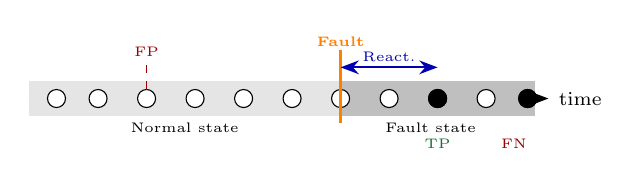
\begin{tikzpicture}[>=Stealth, font=\tiny, scale=0.88]
  \draw[->, thick] (0,0) -- (7.5,0) node[right]{\scriptsize time};
  \fill[gray!20] (0,-0.25) rectangle (4.5,0.25);
  \fill[gray!50] (4.5,-0.25) rectangle (7.3,0.25);
  \node[font=\tiny] at (2.25,-0.42) {Normal state};
  \node[font=\tiny] at (5.8,-0.42) {Fault state};
  \foreach \x in {0.4,1.0,1.7,2.4,3.1,3.8,4.5,5.2,5.9,6.6,7.2} {
    \draw[fill=white, draw=black] (\x,0) circle (0.13);
  }
  \draw[dashed, red!60!black] (1.7,0.13) -- (1.7,0.55);
  \node[red!60!black] at (1.7,0.68) {FP};
  \draw[very thick, orange] (4.5,-0.35) -- (4.5,0.7);
  \node[orange, font=\tiny\bfseries] at (4.5,0.82) {Fault};
  \draw[<->, blue!70!black, thick] (4.5,0.45) -- (5.9,0.45);
  \node[blue!70!black] at (5.2,0.6) {React.};
  \draw[fill=black] (5.9,0) circle (0.13);
  \node[defgreen] at (5.9,-0.65) {TP};
  \draw[fill=black] (7.2,0) circle (0.13);
  \node[red!60!black] at (7.0,-0.65) {FN};
\end{tikzpicture}
\end{center}
\end{notebox}

\end{document}
